\documentclass[border=10pt]{standalone}

\usepackage{tikz}
\usepackage{tikzsymbols}
\usetikzlibrary{calc,patterns,shapes.geometric}

\def\centerarc[#1](#2)(#3:#4:#5){\draw[#1] ($(#2)+({#5*cos(#3)},{#5*sin(#3)})$) arc (#3:#4:#5);}

\begin{document}
	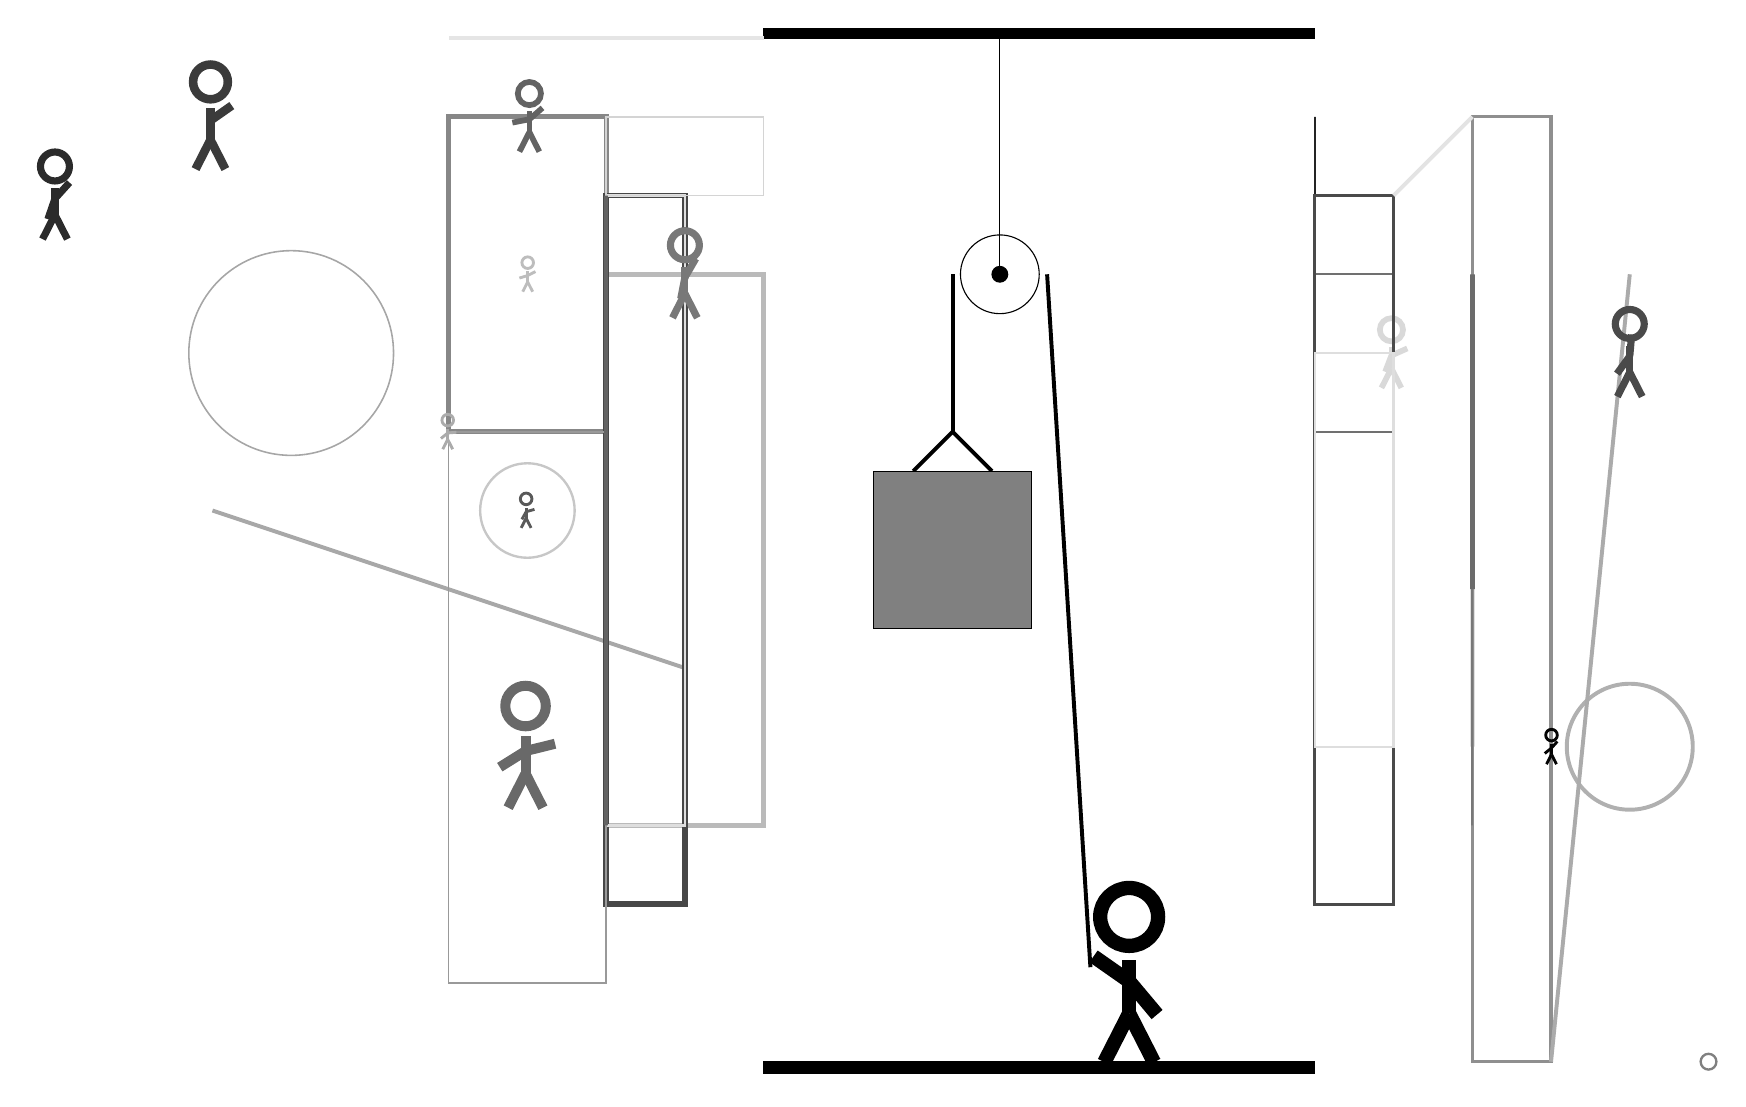
\begin{tikzpicture}
		%%%%% START %%%%%
		
		\draw[fill=black] (-2, 10) rectangle (5, 10.125);
		
		\draw[line width=0.6mm, color=black!47] (-4, 9) rectangle (-6, 5);
		
		\node[line width=0.7mm, color=black!15] at (6, 6) {\Strichmaxerl[4][69][24]};
		\draw[line width=0.2mm, color=black!86] (5, -1) rectangle (5, 9);
		\draw[line width=0.5mm, color=black!34](-3, 2) -- (-9, 4);
		
		\draw[line width=0.7mm, color=black!12] (7, 6) rectangle (7, 1);
		
		\draw[line width=0.3mm, color=black!56] (6, 7) rectangle (5, 5);
		\draw[line width=0.6mm, color=black!27] (-2, 0) rectangle (-4, 7);
		\draw [line width=0.5mm, color=black!31](9, 1) circle (0.8);
		\draw[line width=0.4mm, color=black!44] (7, 9) rectangle (8, -3);
		\draw [line width=0.2mm, color=black!35](-8, 6) circle (1.3);
		
		\node[line width=0.5mm, color=black!26] at (-5, 7) {\Strichmaxerl[2][17][27]};
		\draw[line width=0.5mm, color=black!33](9, 7) -- (8, -3);
		\node[line width=0.2mm, color=black!61] at (-5, 9) {\Strichmaxerl[4][11][41]};
		
		\draw[line width=0.5mm, color=black!10](-2, 10) -- (-6, 10);
		\node[line width=0.5mm, color=black!59] at (-5, 1) {\Strichmaxerl[7][32][14]};
		\draw[line width=0.7mm, color=black!72] (-3, 8) rectangle (-4, -1);
		
		\draw[line width=0.3mm, color=black!13] (-4, 0) rectangle (-3, 8);
		\node[line width=0.3mm, color=black!83] at (-11, 8) {\Strichmaxerl[5][71][48]};
		\draw[line width=0.2mm, color=black!40] (-4, 5) rectangle (-6, -2);
		\node[line width=0.7mm, color=black!65] at (-5, 4) {\Strichmaxerl[2][61][16]};
		\node[line width=0.6mm, color=black!77] at (-9, 9) {\Strichmaxerl[6][90][35]};
		
		\draw[line width=0.2mm, color=black!17] (-2, 8) rectangle (-4, 9);
		\node[line width=0.4mm, color=black!71] at (9, 6) {\Strichmaxerl[5][54][85]};
		\draw [line width=0.3mm, color=black!22](-5, 4) circle (0.6);
		\node[line width=0.3mm, color=black!53] at (-3, 7) {\Strichmaxerl[5][79][60]};
		\draw[line width=0.4mm, color=black!71] (6, -1) rectangle (5, 8);
		\draw [line width=0.3mm, color=black!50](10, -3) circle (0.1);
		\draw[line width=0.5mm, color=black!61] (-4, 8) rectangle (-4, 0);
		\draw[line width=0.5mm, color=black!11](6, 8) -- (7, 9);
		\draw[line width=0.6mm, color=black!58] (7, 7) rectangle (7, 3);
		\draw[line width=0.3mm, color=black!53] (7, 0) rectangle (7, 3);
		
		\node[line width=0.3mm, color=black!33] at (-6, 5) {\Strichmaxerl[2][39][5]};
		\draw[line width=0.3mm, color=black!13] (5, 6) rectangle (6, 1);
		\node[line width=0.7mm, color=black!99] at (8, 1) {\Strichmaxerl[2][39][48]};
		
		\draw (1, 7) circle (0.5);
		\draw[fill=black] (1, 7) circle (0.1);
		\draw (1, 10) -- (1, 7);
		
		\draw[line width=0.5mm] (-0.1, 4.5) -- (0.4, 5.0) -- (0.9, 4.5);
		\draw[fill=black!50] (-0.6, 4.5) rectangle (1.4, 2.5);
		
		\draw[line width=0.5mm] (0.4, 7) -- (0.4, 5.0);
		\centerarc[line width=0.5mm](1, 7)(0:180:0.6);
		\draw[line width=0.5mm](1.6, 7) -- (2.15, -1.8);
		
		\node at (2.6, -1.9) {\Strichmaxerl[10][-35][-50]};
		
		\draw[fill=black] (-2, -3) rectangle (5, -3.15);
		
		%%%%% END %%%%%
	\end{tikzpicture}
\end{document}